%! Author = Giacomo Cavalieri, Nicolò Di Domenico, Nicolas Farabegoli, Linda Vitali
%! Date = 8/5/21

% Preamble
\documentclass[final]{report}

% Packages
\usepackage[utf8]{inputenc}
\usepackage[italian]{babel}
\usepackage{graphicx}
\usepackage{listings}
\usepackage{microtype}
\usepackage{xcolor}
\usepackage{enumitem}
\usepackage{csquotes}
\usepackage{booktabs}
\usepackage{float}
\usepackage[backend=biber]{biblatex}
\usepackage{hyperref}
\usepackage{textcomp}
\addbibresource{ecscala-report.bib}

% custom commands
\def\CC{{C\nolinebreak[4]\hspace{-.05em}\raisebox{.4ex}{\tiny\bf ++}}}
\newcommand{\eg}{\emph{e.g}\ }
\newcommand{\emailaddr}[1]{\href{mailto:#1}{\texttt{#1}}}
\newcommand{\ECS}{\textit{ECS}}
\newcommand{\Entity}{\textit{Entity}}
\newcommand{\Component}{\textit{Component}}
\newcommand{\System}{\textit{System}}
\newcommand{\entity}{\textit{entity}}
\newcommand{\component}{\textit{component}}
\newcommand{\system}{\textit{system}}
\renewcommand{\lstlistingname}{Listato}
\lstset{basicstyle=\ttfamily, showspaces=false, showstringspaces=false}
\definecolor{lightmauve}{rgb}{0.86, 0.82, 1.0}
\lstset{
    language=Scala,
    basicstyle=\footnotesize\ttfamily,
    columns=fixed,
    extendedchars=true,
    breaklines=true,
    tabsize=2,
    prebreak=\raisebox{0ex}[0ex][0ex]{},
    frame=lines,
    showtabs=false,
    showspaces=false,
    showstringspaces=false,
    keywordstyle=\color[rgb]{0.0, 0.0, 1.0},
    commentstyle=\color[rgb]{0.5,0.5,0.5},
    stringstyle=\color[rgb]{0,0.5,0},
    numbers=left,
%numberstyle=\small,
%stepnumber=1,
%numbersep=6pt,
    captionpos=b,
    escapeinside={\%*}{*)}
}

\title{ECScala - A general-purpose ECS framework}
\author{
    Giacomo Cavalieri \\
    \emailaddr{giacomo.cavalieri2@studio.unibo.it}
    \and
    Nicolò Di Domenico \\
    \emailaddr{nicolo.didomenico@studio.unibo.it}
    \and
    Nicolas Farabegoli \\
    \emailaddr{nicolas.farabegoli@studio.unibo.it}
    \and
    Linda Vitali \\
    \emailaddr{linda.vitali2@studio.unibo.it}
}

% Document
\begin{document}
    \maketitle

    \newpage

    \tableofcontents

    \newpage

    \chapter*{Introduzione}
\addcontentsline{toc}{chapter}{Introduzione}
Il progetto ha come obiettivo la realizzazione di un framework che consenta l'implementazione del pattern
architetturale \ECS (Entity Component System).
Questo è un pattern tipicamente usato nel settore videoludico, che favorisce i principi di
\textit{composition over inheritance} e \textit{data-oriented design}.
Due esempi significativi di uso del pattern ECS sono i videogiochi \textit{Overwatch} (2016) e \textit{Minecraft}
(2011).
% TODO: Riguardare talk GDC ed espandere un po' sui vantaggi

I tre concetti chiave di ECS sono:
\begin{itemize}
    \item \Entity: un oggetto distinto che esiste nella simulazione, che non ha dati né comportamenti,
    \eg una palla da biliardo, un nemico di un videogioco, un proiettile, eccetera.
    \item \Component: un elemento che descrive una particolare caratteristica di una \Entity senza descriverne
    l'effettivo comportamento, \eg posizione, velocità, salute, informazioni per il rendering, eccetera.
    \item \System: una funzione che viene eseguita su ogni \Entity che possiede tutti i \Component richiesti e ne
    legge o modifica i loro valori;
    tramite questa si dà l'effettivo comportamento alle \Entity.
    Alcuni esempi di \System possono essere un sistema di rendering che richiede i componenti posizione e immagine,
    un sistema di calcolo dei danni che richiede il componente salute, eccetera.
\end{itemize}

Esistono diverse librerie open source che permettono l'implementazione del pattern \ECS; fra le più importanti risulta
EnTT, libreria scritta in \CC\ usata dal videogioco \textit{Minecraft}.
Nell'ambiente JVM troviamo invece \textit{Artemis} e \textit{Ashley}, entrambe scritte in Java, che però non possono
vantare un uso in applicazioni di rilievo.

Il nostro obiettivo è quindi quello di creare una libreria che faccia della type safety il suo maggior punto di forza,
alla quale si aggiunge un comodo DSL per scrivere codice idiomatico e compatto.
Sebbene le prestazioni siano normalmente d'importanza spesso critica, abbiamo deciso di non realizzare tutte le
ottimizzazioni implementate dalle altre liberie, in quanto esulano dall'obiettivo del corso.
    \chapter{Processo di sviluppo}\label{ch:processo-di-sviluppo}
\section{Metodologia di lavoro}\label{sec:metodologia-di-lavoro}
Il processo di sviluppo adottato dal team si basa sulla versione semplificata di \textit{SCRUM} consigliata dal docente:
sono presenti le figure di \textit{Product Owner} e di \textit{Domain expert}, vengono svolti sprint a cadenza settimanale e si sono redatti
\textit{Product Backlog} e \textit{Sprint Backlog}.
Il team ha applicato il più possibile la tecnica di sviluppo \texttt{test-driven} e largamente sfruttato la modalità collaborativa di \textit{pair programming} che ha
permesso di ottimizzare e rendere più veloce l'implementazione del codice, nonché di individuare rapidamente eventuali bug.

\subsection{Organizzazione degli Sprint}\label{subsec:organizzazione-sprint}
Il primo sprint è stato organizzativo: sono stati identificati gli elementi di base del processo di svilppo, è stata preparata la build del progetto ed è stata prodotta la prima versione del \textit{Product backlog}
secondo i requisiti identificati per il progetto.
È stato inoltre necessario concordare il significato di ``done'' per capire quando uno sprint item potesse considerarsi concluso;
ne è emerso che ciò avviene se e solo se il codice che ne realizza le funzionalità soddisfa i seguenti punti:
\begin{itemize}
    \item i test vengono eseguiti con successo
    \item il codice è ben formattato
    \item è presente la \textit{Scaladoc}
    \item la coverage viene eventualmente decrementata al più del 5\%
    \item il codice prodotto viene controllato e approvato dagli altri membri del gruppo
\end{itemize}
Per quanto riguarda gli sprint successivi, ad inizio settimana il team si è incontrato di persona per la fase di \textit{Sprint Planning} durante la quale, a partire dagli item del \textit{Product Backlog}, è stato prodotto
lo \textit{Sprint Backlog} e sono stati assegnati gli item ai membri.
Al termine di ogni sprint è stata scritta la retrospettiva per verificare l'attuale stato di avanzamento del progetto ed, eventualmente,
posporre gli sprint item non conclusi alla settimana seguente.
Inoltre, ogni membro ha opportunamente aggiornato lo \textit{Sprint Backlog} con l'effort rimanente al completamento del proprio item.

\section{Strumenti utilizzati}\label{sec:strumenti-utilizzati}
A supporto del processo sopra descritto, il team ha principalmente adottato gli strumenti messi a disposizione da \textit{GitHub}: sono state utilizzate le \textit{Issue} per
tenere traccia degli item degli \textit{Sprint Backlog} e assegnarli ai singoli membri;
inoltre, si è ricorso a \textit{Pull Request} da feature branch per permettere la \textit{code review}.
Per avere una visione globale e chiara dell'andamento dello sviluppo, sono stati tracciati e tenuti in versione nel repository del progetto - su file .csv - tutti gli \textit{Sprint Backlog} e il \textit{Product Backlog}.

È stato verificato in modo automatico che il codice prodotto rispettasse i requisiti prestabiliti nella \textit{definition of done} tramite le \textit{GitHub Actions} configurate opportunamente.

In ultimo, si è utilizzato il \textit{Semantic Versioning} per le release.

    \chapter{Requisiti}\label{ch:requisiti}

\begin{table}[H]
    \begin{tabular}{p{0.15\linewidth}p{0.85\linewidth}}
        \toprule
        \textbf{World}     & Contiene più \textit{entity} e i rispettivi \textit{component}. Permette la registrazione di più \textit{system} che utilizza per aggiornare lo stato dei \textit{component} \\
        \textbf{View}      & Rappresenta un sottoinsieme delle \textit{entity} di un \textit{world} con i \textit{component}                                                                              \\
        \textbf{Entity}    & Contiene più \textit{entity} e i rispettivi \textit{component}.                                                                                                              \\
        \textbf{Component} & Rappresenta una particolare caratteristica da modellare per una \textit{entity}                                                                                              \\
        \textbf{System}    & Aggiorna lo stato dei \textit{component} di tutte le \textit{entity} di una determinata \textit{view} secondo una logica definita dall'utilizzatore                          \\
        \bottomrule
    \end{tabular}\label{tab:table}
    \caption{\label{Glossario}}
\end{table}

\section{Business}\label{sec:business}
L'obiettivo è quello di realizzare un framework che permetta di applicare in maniera semplice il pattern ECS\@.

\begin{itemize}
    \item \textit{World} contiene più \textit{entity} e i rispettivi \textit{component}.
    Permette la registrazione di più \textit{system} che utilizza per aggiornare lo stato dei \textit{component}
    \item \textit{View} rappresenta un sottoinsieme delle \textit{entity} di un \textit{world} con i \textit{component}
    specificati
    \item \textit{Entity} è un contenitore di \textit{component} che ne descrivono lo stato
    \item \textit{Component} rappresenta una particolare caratteristica da modellare per una \textit{entity}
    \item \textit{System} aggiorna lo stato dei \textit{component} di tutte le \textit{entity} di una determinata \textit{view}
    secondo una logica definita dall'utilizzatore
\end{itemize}

I requisiti di business individuati sono:
\begin{enumerate}[label=\textbf{\ref{sec:business}.\arabic*}]
    \item \label{itm:b1} Deve essere possibile utilizzare in maniera semplice ed efficiente il pattern ECS
    \item \label{itm:b2} Il framework deve essere sufficientemente flessibile da poter realizzare simulazioni e videogiochi.
    In particolare deve essere possibile:
    \begin{enumerate}[label=\textbf{\ref{itm:b2}.\arabic*}]
        \item \label{itm:bb3} Realizzare una simulazione del moto di palle da biliardo in un tavolo da gioco
    \end{enumerate}
\end{enumerate}

\section{Utente}\label{sec:utente}
I requisiti utente sono sviluppati considerando il punto di vista dello sviluppatore che dovrà utilizzare il framework.
In particolare:
\begin{enumerate}[label=\textbf{\ref{sec:utente}.\arabic*}]
    \item \label{itm:u1} Deve essere possibile creare l'universo che contiene tutte le \textit{entità}
    \item \label{itm:u2} Deve essere possibile creare e rimuovere \textit{componenti}
    \item \label{itm:u3} Deve essere possibile creare e rimuovere \textit{entità}
    \item \label{itm:u4} Deve essere possibile creare \textit{sistemi}
    \item \label{itm:u5} Deve essere possibile utilizzare un DSL per effettuare le operazioni sopra elencate
    \item \label{itm:u6} Per l'utente è importante avere un esempio di utilizzo del framework
\end{enumerate}

\section{Funzionali}\label{sec:funzionali}
I requisiti funzionali, ricavati da quelli utente, sono:
\begin{enumerate}[label=\textbf{\ref{sec:funzionali}.\arabic*}]
    \item \label{itm:f1} Definire un \textit{mondo}
    \begin{enumerate}[label=\textbf{\ref{itm:f1}.\arabic*}]
        \item \label{itm:ff1} Definire delle \textit{viste} che selezionino alcune \textit{entità} del \textit{mondo}
        \item \label{itm:ff2} Far avanzare lo stato del \textit{mondo}, comportando l'aggiornamento delle sue \textit{entità}
    \end{enumerate}
    \item \label{itm:f2} Definire \textit{componenti}
    \item \label{itm:f3} Creare \textit{entità} all'interno di un \textit{mondo}
    \item \label{itm:f4} Rimuovere \textit{entità} dal \textit{mondo} in cui si trovano
    \item \label{itm:f5} Manipolare lo stato delle \textit{entità}
    \begin{enumerate}[label=\textbf{\ref{itm:f5}.\arabic*}]
        \item \label{itm:ff3} Aggiungere \textit{componenti} alle \textit{entità}
        \item \label{itm:ff4} Rimuovere \textit{componenti} dalle \textit{entità}
    \end{enumerate}
    \item \label{itm:f6} Creare \textit{sistemi} per manipolare i \textit{componenti} delle \textit{entità}
    \item \label{itm:f7} Registrare \textit{sistemi} nel \textit{mondo}
    \item \label{itm:f8} Fornire un DSL
    \begin{enumerate}[label=\textbf{\ref{itm:f8}.\arabic*}]
        \item \label{itm:ff5} Definire \textit{sistemi}
        \item \label{itm:ff6} Manipolare \textit{entità}
        \item \label{itm:ff7} Manipolare lo stato del \textit{mondo}
    \end{enumerate}
    \item TODO: demo %TODO: demo progetto
\end{enumerate}


\section{Non funzionali}\label{sec:non-funzionali}
Considerando gli scenari d'uso elencati al punto~\ref{itm:b2}, il sistema deve rispettare il seguente requisito:
\begin{enumerate}[label=\textbf{\ref{sec:non-funzionali}.\arabic*}]
    \item \label{itm:nf1} Aggiornare velocità e posizione di 10'000 \textit{entità} in non più di 10ms
\end{enumerate}


\section{Implementativi}\label{sec:implementativi}
\begin{enumerate}[label=\textbf{\ref{sec:implementativi}.\arabic*}]
    \item \label{itm:i1} Scala 3
    \item \label{itm:i2} Scalatest
    \item \label{itm:i3} JaCoCo per code coverage
    \item TODO %TODO citare eventuali librerie esterne
\end{enumerate}
    \chapter{Design architetturale}\label{ch:design-architetturale}
A seguito dell'analisi dei requisiti definiti nel capitolo precedente, si è realizzato il design architetturale
di massima riportato in Figura.

\begin{figure}[H]
    \centering
    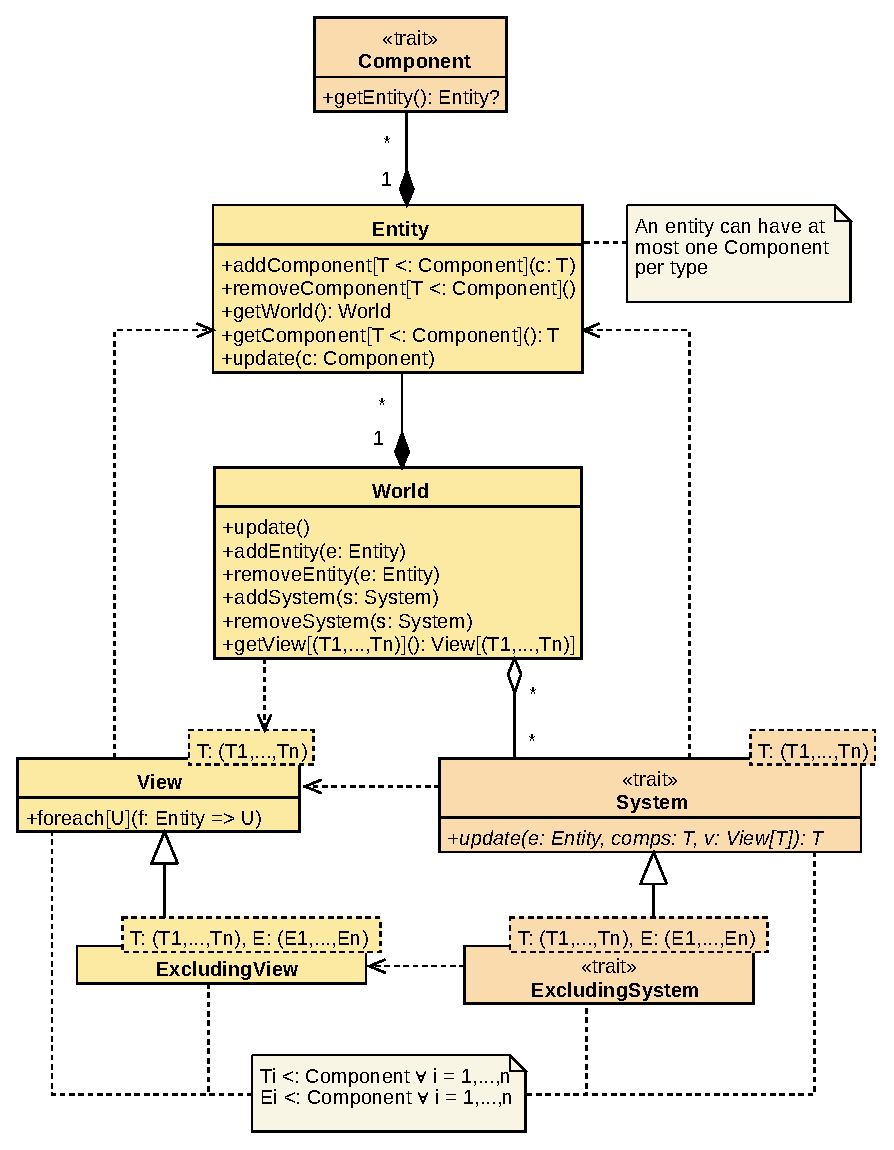
\includegraphics[width=\textwidth]{./img/Architechture}
    \caption{Hello}\label{fig:architecture}
\end{figure}

I principali componenti individuati sono:
\begin{itemize}
    \item \texttt{World}: permette la registrazione e rimozione di \texttt{Entity} e \texttt{System}.
    Il metodo \texttt{update} rappresenta la principale modalità di aggiornamento dello stato di un \texttt{World}: infatti, comporta la modifica dei \texttt{Component} delle \texttt{Entity} registrate secondo la logica descritta dai \texttt{System}.
    Inoltre, è possibile ottenere dal \texttt{World} delle \texttt{View} sulle \texttt{Entity} registrate
    \item \texttt{View}: permette di selezionare le \texttt{Entity} di un \texttt{World} che abbiano tutti i \texttt{Component} specificati
    \item \texttt{ExcludingView}: rappresenta una specializzazione di una \texttt{View} che permette di specificare un ulteriore filtro andando ad indicare i \texttt{Component} che una \texttt{Entity} non deve avere per essere parte della \texttt{View}
    \item \texttt{System}: è un wrapper di una \texttt{View} che, indicando una specifica logica di aggiornamento, si occupa di iterare tutte le \texttt{Entity} selezionate aggiornandone i componenti
    \item \texttt{ExcludingSystem}: in maniera analoga a \texttt{System}, è un wrapper di una \texttt{ExcludingView}
    \item \texttt{Entity}: permette l'aggiunta e rimozione di \texttt{Component} e il loro aggiornamento.
    Non può trovarsi in più \texttt{World} contemporaneamente;
    mantiene un riferimento al \texttt{World} di appartenenza
    \item \texttt{Component}: descrive una particolare caratteristica di un'\texttt{Entity} alla quale viene aggiunto.
    Non può trovarsi in più di un'\texttt{Entity} contemporaneamente;
    mantiene un riferimento all'\texttt{Entity} di appartenenza
\end{itemize}

In Figura è riportato il diagramma di sequenza che descrive le principali interazioni che si verificano quando viene effettuato l'\texttt{update} di un \texttt{World}.

\begin{figure}[H]
    \centering
    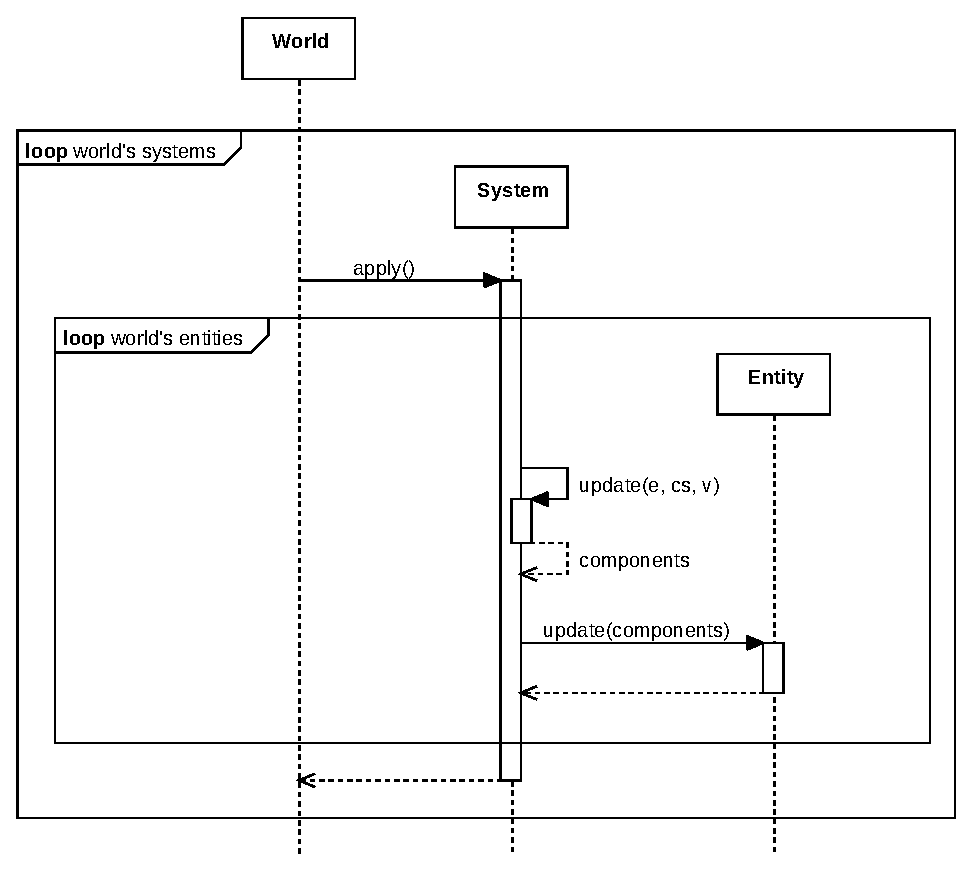
\includegraphics[width=\textwidth]{./img/Sequence}
    \caption{HH}\label{fig:figure}
\end{figure}


    \chapter{Design di dettaglio}\label{ch:design-di-dettaglio}
In seguito alla realizzazione del design architetturale di massima sono state prese
alcune scelte rilevanti relativamente al design di alcune parti del sistema.

\section{Lista di componenti}\label{sec:lista-di-componenti}
Una caratteristica importante della libreria è permettere di specificare nel tipo di un sistema (o una view)
su quali componenti questi operano, così che le stesse firme dei metodi possano guidare il programmatore indicando i
tipi dei componenti trattati.
Così facendo si elimina la necessità di specificare a tempo di esecuzione il tipo di componenti richiesto (come per
esempio è necessario fare nella libreria Ashely~\cite{ashley} che ricorre al passaggio di oggetti \texttt{Class<?>})
permettendo d'intercettare diversi errori a tempo di compilazione.

Realizzare tale funzionalità a livello di compilazione si è rivelato essere una sfida che ha richiesto l’implementazione
delle \texttt{CList}, nonché l’utilizzo di macro per modificare il comportamento del compilatore introducendo controlli
personalizzati.

Una \texttt{CList} (abbreviazione di Components List) è essenzialmente una lista di elementi eterogenei che preserva
informazioni sul tipo di ciascun elemento in maniera simile a una tupla.
Per esempio si osservi il Listato~\ref{lst:lstinputlisting2}: la lista che contiene
i componenti Position e Velocity avrà come tipo~\texttt{Position~\&:~Velocity~\&:~CNil}, permettendo di conoscere il
tipo e la posizione dei suoi elementi.

Nel Listato~\ref{lst:lstinputlisting2} viene mostrato un esempio di utilizzo delle \texttt{CList} nelle~\texttt{View}.
\lstinputlisting[label={lst:lstinputlisting2}, caption=Esempio di utilizzo delle CList.]{code/clist-usage.scala}

L’idea alla base di questa soluzione è ispirata dalle Heterogeneous List della libreria
Shapeless\cite{shapeless}; una differenza significativa sta nel fatto che la definizione di una \texttt{CList} impone un
limite ulteriore sul tipo dei suoi elementi: devono tutti essere sottotipi di \Component, parte dell’implementazione è
riportata al Listato~\ref{lst:lstinputlisting}.

\lstinputlisting[label={lst:lstinputlisting}, caption=Esempio di codice per implementare CList.]{code/clist.scala}

\section{Container di componenti}\label{sec:container-di-componenti}
Come è possibile osservare in Figura~\ref{fig:world-detail}, dal design di dettaglio emerge come
non siano le \Entity stesse a possedere i \Component che vengono loro assegnati.
Infatti, la gestione dei componenti è demandata ad un \texttt{ComponentsContainer}; questo permette
di aggiungere o rimuovere coppie entità-componente o ottenere tutte le entità con uno specifico tipo
di componente.
In questo modo è possibile introdurre in maniera semplice ottimizzazioni nella gestione dei
componenti per rendere la loro iterazione (fondamentale per i \System) quanto più veloce possibile.

Grazie a questa scelta è stato piuttosto semplice modificare l'implementazione del
\texttt{ComponentsContainer} per attuare ottimizzazioni (descritte nel paragrafo~TODO)
necessarie a rispettare il requisito non funzionale~\ref{itm:nf1}.
\begin{figure}
    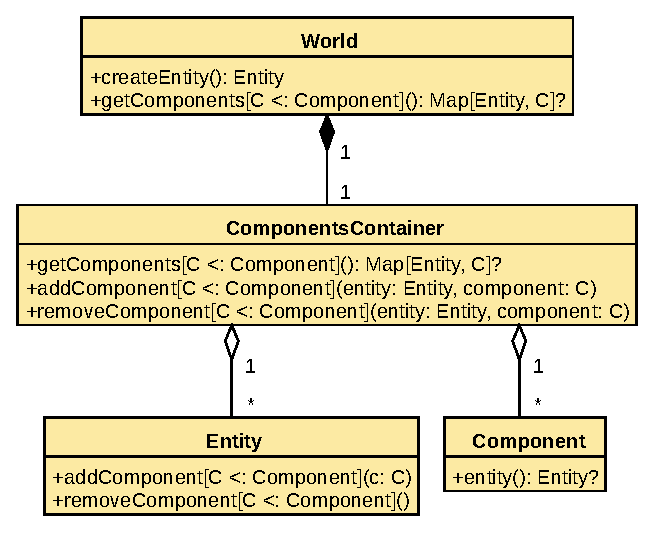
\includegraphics{./img/WorldDetail}
    \caption{Design di dettaglio di World e Entities}
    \label{fig:world-detail}
\end{figure}

\section{Builder dei sistemi}\label{sec:builder-dei-sistemi}
Si è scelto di realizzare il pattern \texttt{Builder} per permettere una creazione di \System
quanto più semplice possibile.
Come mostrato nel diagramma riportato in Figura~TODO il \texttt{SystemBuilder} dispone di diversi metodi per
specificare l'implementazione di alcuni dei metodi del sistema che verrà costruito.
Per ''chiudere'' il \texttt{Builder} e ottenere il nuovo sistema bisogna specificare
l'implementazione del metodo \texttt{update} necessario a stabilirne il comportamento tramite il metodo
\texttt{withUpdate}.

\section{DSL}\label{sec:dsl}

    \chapter{Implementazione}\label{ch:implementazione}
\section{Scala 3}\label{sec:scala-3}
In questa sezione viene esaminato in che modo e dove sono stati utilizzati i nuovi costrutti di Scala 3 nel progetto.

\subsection{Impliciti}\label{subsec:impliciti}

\subsection{Macro}\label{subsec:macro}

\subsection{Context function}\label{subsec:context-function}

\subsection{Match types}\label{subsec:match-types}

\subsection{Type class}\label{subsec:type-class}

\subsection{Extension method}\label{subsec:extension-method}

\subsection{Problemi riscontrati}\label{subsec:problemi-riscontrati}
Nella libreria \texttt{scalatest} è stato riscontrato un bug nella sintassi \texttt{shouldNot typeCheck}.
Tramite questa espressione, dovrebbe essere possibile verificare che una porzione di codice, specificata come stringa,
non compili a causa di un errore nel processo di type checking.
Questo controllo risulta utile nel verificare la corretta destrutturazione delle~\texttt{CList} tramite pattern
matching.
In particolare si è verificato, tramite il codice riportato nel Listato~\ref{lst:lstinputlisting22}, che la
destrutturazione di una \texttt{CList} di dimensione diversa da quanto atteso porti ad un errore di compilazione.
a tal proposito si è definito il test indicato nel Listato~\ref{lst:lstinputlisting22}:
\lstinputlisting[label={lst:lstinputlisting22}, caption=Test per la verifica dell'unpacking delle CList.]
{./code/scalatest-bug.scala}
La prima asserzione verifica che la destrutturazione fallisca se si specificano meno elementi di quanti siano
effettivamente presenti nella lista;
nella seconda si testa lo scenario opposto, ovvero che la destrutturazione fallisca se la lista contiene meno elementi
di quanti ne sono stati specificati nel pattern matching.
Sebbene in entrambi i casi ci si aspetta che le espressioni non compilino a causa di errori nella fase di type checking,
questo non accade e le espressioni vengono erroneamente valutate come valide.
Il bug è stato segnalato agli sviluppatori della libreria mediante una issue~\cite{scalatest-bug}.

Sin dalle prime fasi di sviluppo si è abilitata la modalità di \textit{cross-building}~\cite{cross-building} affinché il
framework venisse compilato anche per Scala.js~\cite{scalajs}.
Questo ha generato una serie di falsi errori all'interno dell'IDE (IntelliJ).
Infatti se si eseguivano i comandi di Sbt per la compilazione del progetto, quest'ultimo non sollevava alcun errore.
A tal proposito è stata aperta una issue~\cite{intellij-issue} sul bug tracker di Jetbrains.
Per una maggiore agilità nella scrittura del codice si è quindi scelto di rimuovere la \textit{cross-building} dal
progetto.

Si segnala che, essendo il rilascio di Scala 3 relativamente recente, non è stato possibile utilizzare
le seguenti librerie per problemi di compatibilità:
\begin{itemize}
    \item Scalafix
    \item Scoverage
    \item ScalaFXML
    \item ScalaMock
\end{itemize}

\section{Benchmarks}\label{sec:benchmarks}
Il requisito non funzionale~\ref{itm:nf1} richiede che il framework operi sotto certi requsiti di prestazioni;
per questo motivo è stato necessario quantificare oggettivamente quali fossero le effettive prestazioni raggiunte.
I benchmark sono uno strumento piuttosto efficace per valutare i tempi di esecuzione (e non solo), fornendo
una stima delle prestazioni in gioco.

Con il termine benchmark si intende un insieme di test specifici per misurare le prestazioni di un software o computer.
Al termine dell'esecuzione del benchmark si ottiene un indice indicativo delle prestazioni che il sistema in oggetto ha
raggiunto.
I benchmark possono essere raggruppati in due categorie:
\begin{itemize}
    \item Sintetici (o microbenckmark): vanno a misurare le prestazioni di alcune parti specifiche di un sistema
    \item Applicativi: misurano le prestazioni complessive di un sistema, ad esempio di un'applicazione
\end{itemize}

Per implementare i microbenchmark necessari alla verifica del requisito non funzionale~\ref{itm:nf1} si è fatto uso del
framework \texttt{Jmh}~\cite{jmh}.
Tale framework consente di definire in modo piuttosto semplice ma altamente configurabile i benchmark.

Scrivere benchmark che misurano correttamente le prestazioni di solo una piccola parte di software è difficile: ci sono
diverse ottimizzazioni che la JVM e l'hardware sottostante sono in grado di fare quando il benchmark esegue solo il
componente, ma tali ottimizzazioni non possono essere effettuate quando il componente è eseguito come parte dell'intera
applicazione, producendo dati falsati.
Implementazioni errate di benchmark possono far credere che le prestazioni dei componenti siano migliori di quanto non
siano in realtà.

Scrivere un benchmark corretto tipicamente evita che la JVM e l'hardware sottostante effettuino ottimizzazioni
durante l'esecuzione del benchmark, che invece potrebbero non essere effettuate a livello complessivo di
applicazione~\cite{jmh:details}.
Grazie a Jmh tutte queste configurazioni sono fatte in automatico e gestite direttamente dal framework, consentendo di
concentrarsi solamente su cosa deve essere testato.

Mediante annotazioni su classi e metodi, è possibile configurare uno o più benchmark: nel
Listato~\ref{lst:lstinputlisting4} è possibile osservare un esempio di configurazione.

\lstinputlisting[label={lst:lstinputlisting4}, caption=Codice per eseguire il setup di un benchmark.]
{code/benchmark.scala}

Come è possibile osservare dal listato, Jmh fornisce molteplici configurazioni che possono essere apportate al
benchmark.
Di particolare rilevanza troviamo: \texttt{@Warmup} e \texttt{@Measurement}.

Con la prima si specifica quante iterazioni devono essere eseguite ``a vuoto'' prima d'iniziare con i test effettivi;
questa procedura risulta necessaria dal momento che quando si esegue per la prima volta un programma sulla JVM, la cache
risulta vuota e quindi il caricamento iniziale delle classi è più lento.
Eseguendo più volte la stessa porzione di codice si ``stabilizza'' la cache, quindi gli accessi successivi saranno più
veloci e uniformi.
Inoltre, nelle JVM HotSpot, l'interprete tiene traccia del numero di volte che un metodo viene eseguito: se tale
numero supera una certa soglia allora viene identificato come \texttt{hot method} (metodo che tipicamente ha dei
loop) e quindi \textit{JIT compiled}.
Chiamate successive all'ottimizzazione risulteranno quindi più veloci ed efficienti.
In questo modo si garantisce che le misurazioni successive alla fase di warm up abbiano valori simili senza essere
influenzate da condizioni esterne.

Con la seconda si specifica quante volte il benchmark debba essere ripetuto.
Per ogni esecuzione viene annotato il tempo impiegato e al termine dell'esecuzione viene riportato il tempo medio che
impiega il test.

\subsection{Risultati}\label{subsec:risultati}
Di seguito sono analizzati i risultati ottenuti dai benchmark delle \View e dei \System.
In Tabella~\ref{tab:benchmark} riportati i risultati riguardanti i \System in cui si può osservare che con $10000$
entità un sistema impiega mediamente cinque millisecondi ad aggiornare le entità, quindi il requisito~\ref{itm:nf1} è
ampiamente rispettato.

\begin{table}[H]
    \centering
    \begin{tabular}{c c}
        \toprule
        Numero entità & Tempo (ms) \\ \midrule
        1024  & $0.502 \pm 0.007$ \\
        2048  & $1.013 \pm 0.018$ \\
        4096  & $2.258 \pm 0.054$ \\
        10000 & $5.413 \pm 0.074$ \\
        \bottomrule
    \end{tabular}
    \caption{\label{tab:benchmark}Risultati benchmark.}
\end{table}

A fronte dei risultati ottenuti dai benchmark si può affermare che il framework fornisce buone prestazioni con un numero
discreto numero di entità.

\section{Suddivisione del lavoro}\label{sec:suddivisione-del-lavoro}
In questa sezione viene illustrata la suddivisione del lavoro e le parti di progetto realizzate da ciascun membro del
gruppo.

\subsection{Farabegoli}\label{subsec:farabegoli}
Il contributo apportato al progetto ha toccato buona parte del core del framework e della demo.
Mi sono infine occupato della gestione del repository, della \textit{Continuous Integration}, dei rilasci del framework
e della qualità del codice.

\subsubsection{World ed Entity}
Una delle parti che ho seguito nelle prime fasi di sviluppo è stata l'implementazione del \World e delle \Entity.
In particolare mi sono occupato di definire l'interfaccia di entrambe le classi e di fornire una prima implementazione
di base.
Ho quindi implementato il codice necessario affinché ogni \Entity avesse un identificativo univoco nel \World.
Infine, mi sono occupato dello sviluppo dei test per la verifica delle classi oggetto d'implementazione.

\subsubsection{View}
Ho definito e implementato parzialmente la classe~\View: in particolare, ne ho realizzato l'interfaccia e fornito una
prima implementazione.
Sempre seguendo un approccio TDD, ho realizzato anche i test necessari alla verifica del corretto funzionamento delle
classi sopra descritte.
Sempre nell'ambito dello sviluppo delle \View, Cavalieri e Di Domenico hanno sviluppato una macro per costruire la
\View in modo che operi sui componenti effettivi passati nel generico;
in questa fase ho contribuito fornendo consigli e suggerimenti per una migliore implementazione del codice.

\subsubsection{Benchmarks}
Come descritto nel requisito non funzionale~\ref{itm:nf1} indica una linea di base delle prestazioni che il framework
deve rispettare;
A tal proposito ho definito una serie di benchmark per misurare le prestazioni di \View, \System e dell'aggiornamento
del World.
Mediante questi benchmark è stato possibile validare il requisito non funzionale sulla base di dati oggettivi.
Per una descrizione più approfondita dei benchmark si faccia riferimento alla Sezione~\ref{sec:benchmarks}.

\subsection{Di Domenico}\label{subsec:nicolò-di-domenico}

Il mio ruolo nel progetto è stato principalmente quello d'implementare le \texttt{View} e i \texttt{System}, nonché
applicare ove necessario eventuali ottimizzazioni per rispettare il requisito non funzionale~\ref{itm:nf1}.

\subsubsection{View}

Essendo le \texttt{View} ed \texttt{ExcludingView} progettate come indicato in Figura~TODO, si è rivelato utile costruire un
iteratore astratto che permettesse di fattorizzare tutto il codice comune.
In particolare si noti come la \texttt{ExcludingView} itera su un sottoinsieme delle entità ritornare dalla stessa
\texttt{View}, che invece non esprime vincoli di esclusione di componenti.
Per questo motivo è stato creato il \texttt{BaseViewIterator}, che si occupa di recuperare dal
\texttt{ComponentsContainer} tutte le mappe che associano ciascuna entità all'istanza (se presente) del componente di
ciascun tipo.
Infine, partendo da tali mappe, si occupa di testare l'appartenenza alla view di ciascuna entità e, in caso affermativo,
estrarne tutti i componenti richiesti.

Una semplice ottimizzazione utilizzata per rendere più veloce l'iterazione di una \texttt{View} consiste nell'individuare
la mappa di componenti con meno elementi;
una volta trovata, si iterano tutte le entità contenute al suo interno e per ognuna si controlla che sia presente in tutte
le altre mappe.
In caso affermativo, si procede all'estrazione di tutti i suoi componenti richiesti.

\subsubsection{System}

Un \texttt{System} è un blocco di codice che può essere aggiunto al \texttt{World} e viene chiamato a ogni aggiornamento
di stato della simulazione.
Ogni \texttt{System} ha due metodi:
\begin{itemize}
    \item \texttt{shouldRun}: metodo booleano che indica se il \texttt{System} dev'essere eseguito
    \item \texttt{update}: metodo che contiene il codice arbitrario da eseguire
\end{itemize}

Su di esso sono stati costruiti \texttt{IteratingSystem} ed \texttt{ExcludingSystem}, due wrapper type-safe
rispettivamente per \texttt{View} ed \texttt{ExcludingView}.
Questi due sistemi definiscono i seguenti metodi:
\begin{itemize}
    \item \texttt{shouldRun}: metodo booleano che indica se l'\texttt{IteratingSystem} dev'essere eseguito
    \item \texttt{before}: metodo eseguito prima di iterare su tutte le entità con i componenti richiesti
    \item \texttt{update}: metodo eseguito per ciascuna entità contenente le operazioni da effettuare sui suoi
    componenti richiesti
    \item \texttt{after}: metodo eseguito dopo aver iterato su tutte le entità con i componenti richiesti
\end{itemize}

Il metodo \texttt{update} deve ritornare una \texttt{CList} dei nuovi componenti;
grazie all'utilizzo delle \texttt{CList} (descritte in dettaglio in TODO) verrà verificato a tempo di compilazione che i
nuovi componenti abbiano lo stesso tipo di quelli su cui opera il sistema.
Per permettere la cancellazione di alcuni dei componenti, è stato implementato un \textit{match type} chiamato
\texttt{Deletable[L~<:~CList]}, come mostrato nel Listato~\ref{lst:deletable};
il suo scopo è quello di permettere l'inserimento in ogni posizione della \texttt{CList} un componente speciale chiamato
\texttt{Deleted}: in tal caso il componente in quella posizione sarà cancellato.

\lstinputlisting[label={lst:deletable}, caption=Implementazione del tipo \texttt{Deletable[L~<:~CList]}]{./code/deletable.scala}

L'\texttt{ExcludingSystem} è completamente analogo all'\texttt{IteratingSystem}, in quanto cambia solo la \texttt{View}
usata per ottenere le entità sulle quali iterare.
Per una maggiore più approfondita sui benchmark si faccia riferimento alla Sezione~\ref{sec:benchmarks}.
    \chapter{Retrospettiva}\label{ch:retrospettiva}
\section{Sprint 1}\label{sec:sprint-1}
\begin{description}
    \item [Svolgimento e sviluppo] Sfruttando il plugin \texttt{sbt-github-actions} sono state generati file per la configurazione della continuous integration.
    I membri del gruppo hanno approfondito la conoscenza del pattern ECS, alcune caratteristiche distintive di Scala 3.
    Si è configurato \texttt{scalafmt} per garantire uno stile uniforme nello sviluppo del progetto.
    Infine, è stato realizzato un design architetturale di massima.
    \item [Considerazioni finali] Lo sprint si è concluso nei tempi previsti e senza evidenziare particolari problematiche.
\end{description}
\section{Sprint 2}\label{sec:sprint-2}
\begin{description}
    \item[Svolgimento e sviluppo] Il secondo sprint è stato incentrato sulla realizzazione del design di dettaglio di World ed Entity.
    Sono stati implementati i principali metodi per l'aggiunta e rimozione dei componenti.
    È stata anche implementata la struttura dati \texttt{IterableMap}.
    \item[Considerazioni finali] Uno dei product backlog item (As a framework user I want to define World's views) non è stato concluso
    in tempo e pertanto è stato rimandato allo sprint successivo.
    I rimanenti product backlog item sono stati conclusi nei tempi prestabiliti.
\end{description}
\section{Sprint 3}\label{sec:sprint-3}
\begin{description}
    \item[Svolgimento e sviluppo] Durante lo sprint è stata completata l'implementazione delle \texttt{View} e realizzata una prima versione del DSL\@.
    Poiché grazie all'implementazione delle \texttt{View} il cuore della libreria può considerarsi concluso, sono stati realizzati dei benchmark
    per verificare il rispetto del requisito non funzionale~\ref{itm:nf1} ottenendo discreti risultati preliminari.
    \item[Considerazioni finali] Al termine dello sprint è emerso un problema implementativo che ha comportato un aumento significativo nello sforzo
    stimato per completare due dei backlog item (As a framework user I want to define and use Systems e As a framework user I want to update the World's state);
    perciò è stato spostato allo sprint successivo.
\end{description}
\section{Sprint 4}\label{sec:sprint-4}
\begin{description}
    \item[Svolgimento e sviluppo] Il team si è focalizzato sulla realizzazione dei \texttt{System} i quali hanno richiesto uno sforzo condiviso e collaborazione fra i vari membri.
    In questo modo
    è stato possibile risolvere le problematiche emerse senza ulteriori ritardi.
    Allo stesso tempo si è proseguito con la realizzazione del DSL\@.
    \item[Considerazioni finali] Lo sprint si è concluso senza problemi da evidenziare.
\end{description}
\section{Sprint 5}\label{sec:sprint-5}
\begin{description}
    \item[Svolgimento e sviluppo] Non avendo fin'ora riscontrato ritardi significativi nello sviluppo, il team ha deciso di aggiungere meno item allo sprint per poter conciliare impegni accademici.
    Sono stati implementati \texttt{ExcludingView} ed \texttt{ExcludingSystem} ed è stato arricchito il DSL per permettere l'aggiunta di \texttt{System} e la rimozione di \texttt{Component}.
    \item[Considerazioni finali] Lo sprint si è concluso evidenziando incosistenze nella sintassi del DSL che saranno corrette nel prossimo sprint.
    Inoltre, intendiamo fare refactoring dell'interfaccia di \texttt{World} che secondo noi ha margini di miglioramento ma essendo una modifica consistente non poteva essere completata in questo sprint.
\end{description}
\section{Sprint 6}\label{sec:sprint-6}
\begin{description}
    \item[Svolgimento e sviluppo] Lo sprint si è focalizzato principalmente sulla definizione dell'architettura per la demo.
    Inoltre, sono state apportate migliorie alla sintassi del DSL ed è stata semplificata l'interfaccia del \texttt{World}.
    Infine, è stato effettuato il primo rilascio della libreria dal momento che sono state implementate tutte le funzionalità minime necessarie.
    \item[Considerazioni finali] Abbiamo deciso di spostare uno degli sprint item (Refactor World's interface) a quello successivo, in quanto ritenuto di bassa priorità.
\end{description}
\section{Sprint 7}\label{sec:sprint-7}
\begin{description}
    \item[Svolgimento e sviluppo] Lo sprint ha avuto come obiettivo principale la realizzazione della demo.
    Inoltre è stato effettuato il refactoring della classe \texttt{World} e le corrispondenti parti nel DSL\@.
    \item[Considerazioni finali] Sono stati spostati allo sprint successivo gli item "Refactor World's interface" e "As a framework user I would higly appreciate a handy DSL to perform these operations".
\end{description}
\section{Sprint 8}\label{sec:sprint-8}
\begin{description}
    \item[Svolgimento e sviluppo]
    \item[Considerazioni finali]
\end{description}

    \printbibliography

\end{document}